\documentclass[12pt,a4paper,twoside]{article}
% Adapted from the supplied ReportTemplate: article, 25 mm margins and
% separate individual/team work. Two columns are requested for this report.
\usepackage[a4paper,left=25mm,right=25mm,top=25mm,bottom=25mm]{geometry}
\usepackage{fontspec}
\usepackage[british]{babel}
\usepackage{amsmath,amssymb,graphicx,booktabs,array}
\usepackage{caption,subcaption}
\usepackage[square,comma,numbers,sort&compress]{natbib}
\usepackage[hidelinks]{hyperref}
\usepackage{url,fancyhdr,microtype,placeins}
\graphicspath{{figures/}}
\setlength{\columnsep}{6mm}
\setlength{\parindent}{1em}
\setlength{\parskip}{0pt}
\setlength{\headheight}{14pt}
\setlength{\emergencystretch}{1.5em}
\captionsetup{font=small,labelfont=bf}
\captionsetup[subfigure]{font=small}
\setlength{\tabcolsep}{4pt}
\renewcommand{\arraystretch}{1.08}
\renewcommand{\topfraction}{0.92}
\renewcommand{\bottomfraction}{0.85}
\renewcommand{\textfraction}{0.08}
\renewcommand{\floatpagefraction}{0.75}
\setcounter{topnumber}{3}
\setcounter{bottomnumber}{2}
\setcounter{totalnumber}{5}
\pagestyle{fancy}
\fancyhf{}
\fancyfoot[C]{\thepage}
\renewcommand{\headrulewidth}{0pt}
\renewcommand{\footrulewidth}{0pt}
\urlstyle{tt}
\Urlmuskip=0mu plus 1mu
\DeclareRobustCommand{\code}[1]{\begingroup\small\nolinkurl{#1}\endgroup}
\makeatletter
\renewcommand\section{\@startsection{section}{1}{\z@}%
  {-2.4ex plus -.6ex minus -.2ex}{1.1ex plus .2ex}%
  {\normalfont\normalsize\bfseries}}
\renewcommand\subsection{\@startsection{subsection}{2}{\z@}%
  {-1.9ex plus -.5ex minus -.2ex}{.8ex plus .2ex}%
  {\normalfont\normalsize\bfseries}}
\makeatother
\newcommand{\R}{\mathbb{R}}
\title{\Large Lab 5: Individual Assignment (D1--D2)}
\author{Ruihang Liu\\[2pt]\normalsize Student ID: 24020036043\\
  \normalsize Team Fullcans\\
  \normalsize Ocean University of China}
\date{}
\hypersetup{pdftitle={Lab 5: Individual Assignment (D1--D2)},
  pdfauthor={Ruihang Liu}}

\begin{document}
\makeatletter
\twocolumn[
\begin{@twocolumnfalse}
\maketitle
\vspace{-2em}
\begin{center}\small
\url{https://github.com/monessss/2026Fall-Robotics-Integrated-Project}\par
Exercises: \url{https://vnav.mit.edu/labs_2023/lab5/exercises.html}
\end{center}
\vspace{0.3em}
\end{@twocolumnfalse}
]
\makeatother
\thispagestyle{fancy}

\section{D1: Perspective projection of a sphere}
The optical centre is the origin. With focal length one, principal point
$(0,0)$, unit pixel scale and zero skew, a point $(x,y,z)^\top$ with $z>0$
projects to $(u,v)=(x/z,y/z)$. Define
\begin{equation}
  w=(u,v,1)^\top,\qquad P(\lambda)=\lambda w,\quad \lambda>0.
  \label{eq:ray}
\end{equation}
For a sphere of radius $r$ centred at $c=(0,0,d)^\top$, a ray intersects the
surface when
\begin{equation}
  (u^2+v^2+1)\lambda^2-2d\lambda+d^2-r^2=0.
\end{equation}
The condition $d>r+1$ places the sphere entirely beyond the image plane
$z=1$. The discriminant condition is
\begin{equation}
  d^2-(d^2-r^2)(u^2+v^2+1)\geq0.
\end{equation}
Both roots are positive whenever they exist, since $d>r$ and their sum and
product are positive. Thus the projected region and its tangent-ray boundary
are
\begin{align}
  u^2+v^2&\leq\frac{r^2}{d^2-r^2},\\
  u^2+v^2&=\frac{r^2}{d^2-r^2}.
  \label{eq:circle}
\end{align}
The image is a disc of radius $r/\sqrt{d^2-r^2}$. The commonly used value
$r/d$ is only its far-distance approximation.

For a general centre $c=(c_x,c_y,c_z)^\top$, assume first that the camera is
outside the sphere. Substitution of \eqref{eq:ray} gives
\begin{equation}
  \|w\|^2\lambda^2-2(c^\top w)\lambda+\|c\|^2-r^2=0.
\end{equation}
Writing $k=\|c\|^2-r^2>0$, tangency requires
\begin{equation}
  (c_xu+c_yv+c_z)^2=k(u^2+v^2+1).
  \label{eq:conic}
\end{equation}
This is a conic, but visibility still requires positive ray depth; a real
algebraic contour behind the camera is not a visible forward projection.
If $\|c\|<r$, every forward ray meets the surface, so no bounded exterior
silhouette is obtained. At $\|c\|=r$, the nonzero ray intersection is positive
only when $c^\top w>0$; this is a degenerate case of the exterior-contour model.

For a sphere entirely in front, $c_z>r$, let
$q=c_z^2-r^2>0$ and $\rho=\sqrt{c_x^2+c_y^2}$. Rotate the image axes so that
$u'$ follows $(c_x,c_y)$; if $\rho=0$, either image-axis direction is suitable.
Since $k=q+\rho^2$, completing the square yields
\begin{align}
  u'_0&=\frac{\rho c_z}{q},\\
  q(u'-u'_0)^2+kv'^2&=\frac{r^2k}{q}.
  \label{eq:ellipse}
\end{align}
The contour is an ellipse, with semi-axes
\begin{equation}
  a_\parallel=\frac{r\sqrt{k}}{q},\qquad
  a_\perp=\frac{r}{\sqrt q}.
\end{equation}
Its centre in the original image coordinates is
$c_z(c_x,c_y)^\top/q$, which generally differs from the projection of the
sphere centre. When $\rho=0$, the two semi-axes coincide and
\eqref{eq:circle} is recovered.

\begin{figure}[tb]
  \centering
  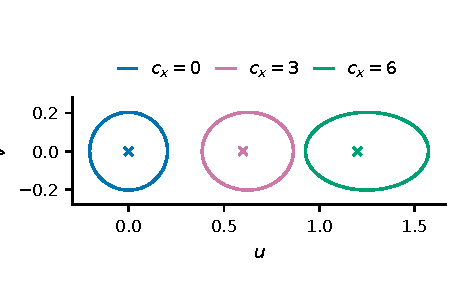
\includegraphics[width=\columnwidth]{sphere_analytic.pdf}
  \caption{Analytic sphere silhouettes for $r=1$, $c_z=5$ and three horizontal
    centre offsets. Crosses mark the projected sphere centres; an off-axis
    silhouette is elliptical and its centre shifts outward.}
  \label{fig:sphere}
\end{figure}

Figure~\ref{fig:sphere} illustrates this offset. More generally, for an external
camera, $c_z=r$ with $\rho>0$ gives a parabolic contour; $|c_z|<r$ gives a
hyperbolic algebraic contour, of which only the positive-depth part is visible.
If $c_z\leq-r$, no sphere point has strictly positive depth. These cases explain
why the bounded-ellipse result must retain the condition $c_z>r$.

\section{D2: Vanishing points and parallel image lines}
Let a spatial line be
\begin{equation}
  P(\lambda)=p_0+\lambda a,\qquad a=(a_x,a_y,a_z)^\top\ne0.
\end{equation}
Its finite image coordinates satisfy
\begin{equation}
  \pi(P(\lambda))=
  \left(\frac{p_{0x}+\lambda a_x}{p_{0z}+\lambda a_z},
        \frac{p_{0y}+\lambda a_y}{p_{0z}+\lambda a_z}\right).
\end{equation}
If $a_z\ne0$, choose $\lambda\to+\infty$ for $a_z>0$ or
$\lambda\to-\infty$ for $a_z<0$, so that depth tends to positive infinity.
The vanishing point is
\begin{equation}
  v_\infty=(a_x/a_z,\ a_y/a_z).
  \label{eq:vp}
\end{equation}
It depends on the common direction, not on $p_0$. In homogeneous coordinates,
$\widetilde v_\infty\sim(a_x,a_y,a_z)^\top$; $a_z=0$ places it at infinity.
Geometrically, each spatial line and the optical centre span a plane. Two
such planes for parallel lines share the direction $a$, which produces the
same vanishing point.

For the parallelism statement, assume that both spatial lines have visible
parts, neither passes through the optical centre, and their image lines are
distinct. Their images are parallel if and only if $a_z=0$.
To prove sufficiency, set $a_z=0$: depth on each line is constant and positive,
so its image has direction proportional to $(a_x,a_y)^\top$. Both images
therefore have the same direction. For necessity, if $a_z\ne0$, both image-line
extensions contain the finite point \eqref{eq:vp}; distinct lines sharing a
finite point cannot be parallel.

The distinct-image condition matters. The different spatial lines
$L_1(t)=(t,1,1)$ and $L_2(t)=(t,2,2)$ both project to $v=1$. Such coincident
images must not be treated as a counterexample to the stated condition.

\end{document}
